\chapter{Technology studies}

The technology studies covers the studies leading up to the design and implementation. The technology studies help give an overview of how to realise the power line communication bus by providing good knowledge into the theory needed. During the technology studies the procedure were:
\begin{enumerate}
\item Discover literature
\item Create overview
\item Read and understand
\item Experiment
\end{enumerate}


\section{Protocol and communications}


\section{Clock and data recovery}
Normally a data transmission consists of two elements, clock and data. In this system that is not possible and therefore the area of clock and data recovery was investigated.

\subsection{What is clock recovery?}
Clock recovery is achieved essentially by extracting the clock from the incoming data stream. Due to the level shifts of the bitstream the clock is carried in the data.
\fixme{Skrives noget mere til hvad clock recovery er}

\subsection{The Phase-locked loop}
The phase-locked loop(PLL) comes in a large variety of designs but they all have one common conceptual diagram. A PLL consists of a phase-detector, a filter and a voltage controlled oscillator(VCO). Optionally it can contain a clock divider as well to speed up the VCO clock. Below on figure \ref{fig:conceptualpll} is shown the structure of the conceptual PLL.

\begin{figure}[H]
	\centering
	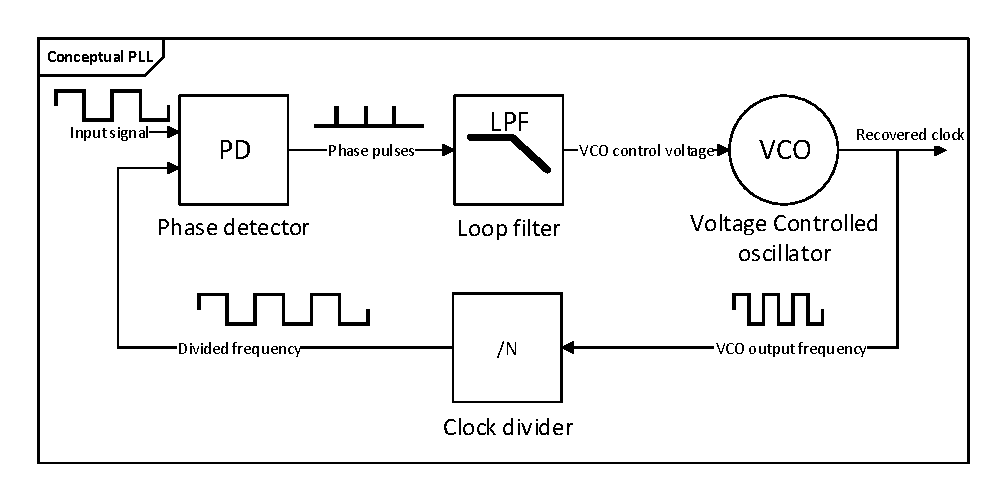
\includegraphics[width=.9\textwidth]{billeder/10technologystudies/conceptualpll}
	\caption{Conceptual PLL}
	\label{fig:conceptualpll}
\end{figure}

\subsubsection{Phase detector}
The phase detector takes in


\subsubsection{Loop filter}

\subsubsection{Voltage controlled oscillator}

\subsubsection{Clock divider}



